\chapter{Interpretations of the results}

\lettrine{D}{}ata yield in \SI{36.4}{\ifb}, presented in the previous chapter, are in agreement with prediction of the SM. This chapter quantifies this level of agreement introducing appropiate test statistics allowing to set model independent, regardless of the model considered, and model dependent, within the Minimal DM model, upper limits.

\section{The profiled likelihood ratio}
In \Sect{\ref{sec:likelihood}} the Likelihood function was defined as a function of the POI $\mu$~\cite{Cowan}.
A very common procedure to establish discovery (or exclusion) in particle physics is based on a likelihood ratio as a test statistic. Indeed, to test an hypothesized value of $\mu$ the \emph{profiled likelihood ratio} which is used as the principal statistical parameter in this analysis, has been considered.
\begin{equation}
  \lambda(\mu) = \frac {\mathfrak{L}(\mu,\hat{\hat{\theta}})}{\mathfrak{L(\hat{\mu},\hat{\theta})}}
  \label{eqn:profiled}
\end{equation}
where the numerator, $\hat{\hat{\theta}}$ conditional maximum-likelihood estimator (MLE) of $\theta$, or the value which maximies $\mathfrak{L}$ for a given $\mu$ (therefore, it is a function of $\mu$, and the denominator is the maximized, unconditionally by fixing no parameters, likelihood function. \Eqn{\ref{eqn:profiled}} is a rescaling of the likelihood function: 

\subsection{The $t_\mu$ test statistic}
The profiled likelihood ratio $\lambda(\mu)$ is constrained to vary between 0 and 1 so that it is useful to define the corresponding $\tmu$ statistic as 
\begin{equation}
  t_{\mu} = -2 \log{\lambda(\mu)}
\end{equation}
which can be used to build a statistic to measure the discrepancy between data and the hypothesis where higher value of $t_{\mu}$ correspond to higher disagreement. The \p can also be evaluated, and its correspondance to $t_{\mu}$ is pointed out in \Fig{\ref{pvalue}}, as:
\begin{equation}
 p_{\mu}=\int_{t_{\mu,\textup{obs}}}^\infty f\left(t_\mu \vert \mu\right) dt_\mu
 \label{eqn:pdatmu}
\end{equation}

where $t_{\mu,\textup{obs}}$ is the value of $t_\mu$ observed from data and $f\left(t_\mu \vert \mu\right)$ is the probability density function of $t_\mu$ under the assumption of the POI value $\mu$. One can often assume that presence of new signal can only increase the mean event rate, which for a counting experiment can be evaluated as $E[n] = \mu s + b$ where $s$ are the signal events and $b$ is the background, so that we can consider parameter $\mu$ as positive so that an alternative test statistic $\tilde{t}_\mu$ can be defined. For a model in which $\mu>0$, if one finds that $\hat{\mu}<0$, the best level of agreement must be for $\mu=0$.

Note that $f\left(t_\mu \vert \mu\right)$ in \Eqn{\ref{eqn:pdatmu}}, like all the $f$ distribution in this Section, is unknown, because we miss the real POI which is crucial to its determination. According to Wilks' theorem, the distribution of $f(t_\mu \vert \mu)$ is known in the case of a large statistics an it follows a one-degree of freedom (in case of one POI) $\chi^2$ distribution, regardless of the values taken by the nuisance parameters, see~\cite[\Sect{3}]{Cowan}, so that $f$ is expressed in term of certain asymptotic formul\ae~ in the limit of large samples. Alternatively one can obtain it by performing several pseudo-experiment, i.e. \emph{toys}, to get the right distribution expression even if they're always time expensive.

\begin{figure}[tp]
\centering
\subfloat[][]
{\includegraphics[width=.4\textwidth]{monophoton/pvaluea}}
\subfloat[][]
{\includegraphics[width=.416\textwidth]{monophoton/pvalueb}}
\caption{(\emph{a}) Relation between \p and $t_{\mu,\textup{obs}}$. (\emph{b}) Relation between the significance $Z$ and \p for a gaussian distribution $\varphi(x)$.}
\label{pvalue}
\end{figure}

\subsection{Test statistics for discovery and exclusion fit}
Without any observed excess of events in one or more SR(s), two methods set exclusion
limits on specific signal models. These two fit strategies, complementary to the background only fit described {\bf above}, are the discovery fit, or model-independent and the exclusion fit model-dependent. Both fit are used to set upper limits on the POI, i.e. the number of events in case of discovery and the visible cross section for exclusion, by varying its value whithin a certain range and then interpolating for which POI value one finds \SI{95}{\percent} exclusion. For this reason, setting an upper limit is also called \emph{hypotest inversion}.

\subsubsection{The $q_0$ test for discovery of a positive signal}
When searching for new physics phenomena typically one would put constraints on potential new physiscs. Indeed, in a discovery fit the purpose is to set model-independent \SI{95}{\percent} CL upper limits on the number of Beyond Standard Model (BSM) events in SR. For no signal model in particular anyone can estimate the number of signal events predicted in a particular SR, in our case the already defined ``fiducial region'', and see wether a certain model has been excluded by current data or not.

In this scenario rejecting the $\mu = 0$ hypothesis leads to the discovery of a new signal.  An appropriate test, the $q_0$ test statistic, is therefore defined as follows:
\begin{equation}
q_0=
\left\{
\begin{aligned}
-2\log{\lambda(0)}\quad &\text{if}\quad \hat{\mu}\ge0\\
 0 \qquad&\text{if}\quad \hat{\mu}<0
\end{aligned}
\right.
\end{equation} 

Data shows lack of agreement with the background only hypothesis ($\hat{\mu}=0$), only if $q_0\ne0$. Using the observed value of $q_0$ one can quantify the level of disagreement between the data and the null hypothesis not so much unlike for the $t_\mu$ case:
\begin{equation}
 p_{\mu}=\int_{q_{0,\textup{obs}}}^\infty f\left(q_0 \vert 0\right) dq_0
 \label{eqn:pdaq0}
\end{equation}

\subsubsection{The $q_\mu$ test for model dependent upper limits}
This fit strategy is used with the objective of studying a specific signal model. Again, with no relevant excess of events proved by the background only fit exclusion limits can be performed for    setting upper limit on the visible cross section of the model being tested. The signal sample must be added to every CRs and not only in the SR, in order to take into account any posssible signal contamination in the CRs. Note that this test is useful even in case of excess of events for which can be used to measure properties such as the signal strength.

Like for the model independent fit, a suitable test statistic can be defined for the model independent fit as well, in a very similar way. However, now the null hypothesis is the signal+background coexisting in the SR because a signal is supposed to be tested against the back. Therefore the $q_\mu$ test statistic is defined as:
\begin{equation}
q_\mu=
\left\{
\begin{aligned}
-2\log{\lambda(0)}\quad &\text{if}\quad \hat{\mu}\le\mu\\
 0 \qquad&\text{if}\quad \hat{\mu}>\mu
\end{aligned}
\right.
\end{equation} 
Once again the relation between $q_\mu$ and the \p is straighforward:
\begin{equation}
 p_{\mu}=\int_{q_{\mu,\textup{obs}}}^\infty f\left(q_\mu \vert \mu\right) dq_\mu
 \label{eqn:pdaqmu}
\end{equation}

\subsection{Experimental sensitivity}
\label{sec:sensitivity}
To characterize the sensitivity of an experiment, the significance obtained from a single dataset is irrelevant. The expected (or median) significance which allows to reject different values of $\mu$ is more useful. In a discovery analysis one would like to know the median significance with which one would reject the background-only null hypothesis and for exclusion the median with which one rejects a nonzero value of $\mu$.

The median significance is obtained by replacing the ensamble of simulated data set with a single representative one, the so-called Asimov data set which it is easy to obtain the median values of $q_0$ and $q_\mu$.

The sensitivity of an experiment is illustrated in \Fig{\ref{fig:medianq}} which shows the PDF for $q_\mu$ assuming an observed (tested) value of $\mu$ and an expected value of $\mu'$ retrieved from certain asymptotic formul\ae~ valid in the case of large samples~\cite{Cowan}. Analogous consideration can be made for the discovery analysis by replacing $q_\mu$ with the corresponding $q_0$. The sensitivity of an experiment can be characterized by giving the \p corresponding to the median $q_\mu$, assuming $\mu=\mu'$. 

When the distribution of the strenght parameters $\mu'$ gets shifted to higher values, so does the median $q_\mu$. From \Eqn{\ref{eqn:pdaq0}} and \Eqn{\ref{eqn:pdaqmu}} it is clear that \p is pushed towards lower values. Now the hypotest inversion is finally revealed. What the fitting procedure achieved is to scan several values of $\mu$ and evaluate the median \p assuming $\mu'$. The computed upper limit is therefore the value of $\mu$ for which \p gets under the threshold of \num{0.05}.

In the context of exclusion limits, the $\cls$ statistic is mostly used replacing the \p. $\cls$ being derived from the \p is defined as:
\begin{equation}
	\cls=\frac{\text{p-value}(H_0)}{1-\text{p-value}(H_1)}
\end{equation}

Upper limits are then set for the value when $\cls$ is computed to be below the $0.05$ threshold.

\begin{figure}[pt]
\centering
\includegraphics[width=0.5\textwidth]{interpretations/medianq}
\caption{Representation of the situation described in \Sect{\ref{sec:sensitivity}}. The observed distribution $f\left(q_\mu \vert \mu \right)$ is overlapped with the median $f\left(q_\mu \vert \mu' \right)$ given by the asimptotic formul\ae~ according to which it has the form of an half chi squared distribution. The median $q_\mu$ is computed assuming the alternate value $\mu'$ and the result is used to calculate the \p for distribution $f\left(q_\mu \vert \mu \right)$.}
\label{fig:medianq}
\end{figure}

\section{Model-independent limit}

%\section{prova}
%\begin{figure}[tp]
\centering
{\fontfamily{phv}\selectfont  
\small
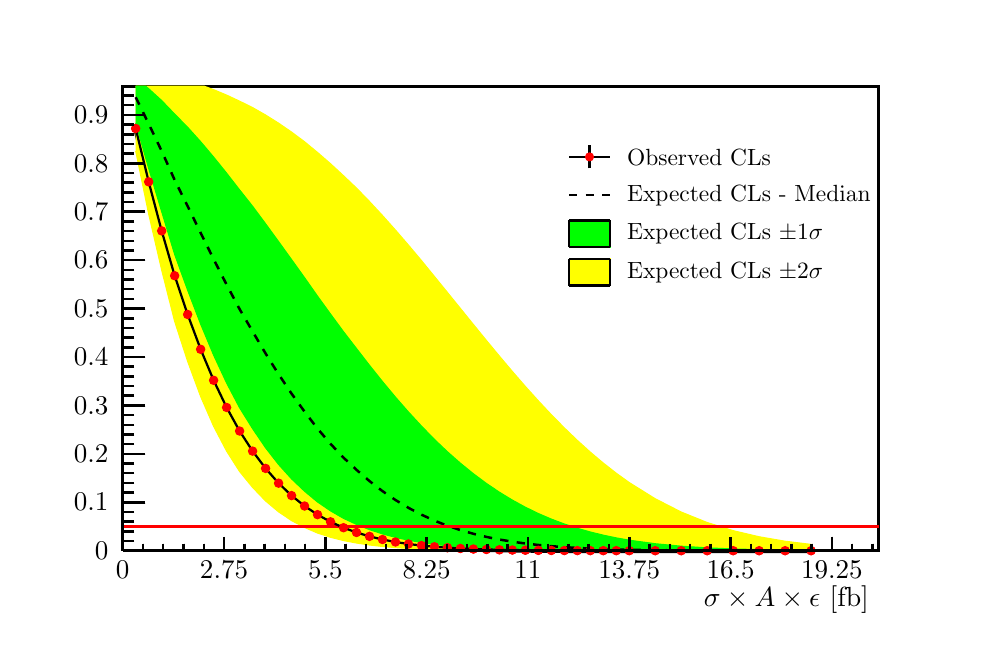
\begin{tikzpicture}[scale=0.6]
\pgfdeclareplotmark{cross} {
\pgfpathmoveto{\pgfpoint{-0.3\pgfplotmarksize}{\pgfplotmarksize}}
\pgfpathlineto{\pgfpoint{+0.3\pgfplotmarksize}{\pgfplotmarksize}}
\pgfpathlineto{\pgfpoint{+0.3\pgfplotmarksize}{0.3\pgfplotmarksize}}
\pgfpathlineto{\pgfpoint{+1\pgfplotmarksize}{0.3\pgfplotmarksize}}
\pgfpathlineto{\pgfpoint{+1\pgfplotmarksize}{-0.3\pgfplotmarksize}}
\pgfpathlineto{\pgfpoint{+0.3\pgfplotmarksize}{-0.3\pgfplotmarksize}}
\pgfpathlineto{\pgfpoint{+0.3\pgfplotmarksize}{-1.\pgfplotmarksize}}
\pgfpathlineto{\pgfpoint{-0.3\pgfplotmarksize}{-1.\pgfplotmarksize}}
\pgfpathlineto{\pgfpoint{-0.3\pgfplotmarksize}{-0.3\pgfplotmarksize}}
\pgfpathlineto{\pgfpoint{-1.\pgfplotmarksize}{-0.3\pgfplotmarksize}}
\pgfpathlineto{\pgfpoint{-1.\pgfplotmarksize}{0.3\pgfplotmarksize}}
\pgfpathlineto{\pgfpoint{-0.3\pgfplotmarksize}{0.3\pgfplotmarksize}}
\pgfpathclose
\pgfusepathqstroke
}
\pgfdeclareplotmark{cross*} {
\pgfpathmoveto{\pgfpoint{-0.3\pgfplotmarksize}{\pgfplotmarksize}}
\pgfpathlineto{\pgfpoint{+0.3\pgfplotmarksize}{\pgfplotmarksize}}
\pgfpathlineto{\pgfpoint{+0.3\pgfplotmarksize}{0.3\pgfplotmarksize}}
\pgfpathlineto{\pgfpoint{+1\pgfplotmarksize}{0.3\pgfplotmarksize}}
\pgfpathlineto{\pgfpoint{+1\pgfplotmarksize}{-0.3\pgfplotmarksize}}
\pgfpathlineto{\pgfpoint{+0.3\pgfplotmarksize}{-0.3\pgfplotmarksize}}
\pgfpathlineto{\pgfpoint{+0.3\pgfplotmarksize}{-1.\pgfplotmarksize}}
\pgfpathlineto{\pgfpoint{-0.3\pgfplotmarksize}{-1.\pgfplotmarksize}}
\pgfpathlineto{\pgfpoint{-0.3\pgfplotmarksize}{-0.3\pgfplotmarksize}}
\pgfpathlineto{\pgfpoint{-1.\pgfplotmarksize}{-0.3\pgfplotmarksize}}
\pgfpathlineto{\pgfpoint{-1.\pgfplotmarksize}{0.3\pgfplotmarksize}}
\pgfpathlineto{\pgfpoint{-0.3\pgfplotmarksize}{0.3\pgfplotmarksize}}
\pgfpathclose
\pgfusepathqfillstroke
}
\pgfdeclareplotmark{newstar} {
\pgfpathmoveto{\pgfqpoint{0pt}{\pgfplotmarksize}}
\pgfpathlineto{\pgfqpointpolar{44}{0.5\pgfplotmarksize}}
\pgfpathlineto{\pgfqpointpolar{18}{\pgfplotmarksize}}
\pgfpathlineto{\pgfqpointpolar{-20}{0.5\pgfplotmarksize}}
\pgfpathlineto{\pgfqpointpolar{-54}{\pgfplotmarksize}}
\pgfpathlineto{\pgfqpointpolar{-90}{0.5\pgfplotmarksize}}
\pgfpathlineto{\pgfqpointpolar{234}{\pgfplotmarksize}}
\pgfpathlineto{\pgfqpointpolar{198}{0.5\pgfplotmarksize}}
\pgfpathlineto{\pgfqpointpolar{162}{\pgfplotmarksize}}
\pgfpathlineto{\pgfqpointpolar{134}{0.5\pgfplotmarksize}}
\pgfpathclose
\pgfusepathqstroke
}
\pgfdeclareplotmark{newstar*} {
\pgfpathmoveto{\pgfqpoint{0pt}{\pgfplotmarksize}}
\pgfpathlineto{\pgfqpointpolar{44}{0.5\pgfplotmarksize}}
\pgfpathlineto{\pgfqpointpolar{18}{\pgfplotmarksize}}
\pgfpathlineto{\pgfqpointpolar{-20}{0.5\pgfplotmarksize}}
\pgfpathlineto{\pgfqpointpolar{-54}{\pgfplotmarksize}}
\pgfpathlineto{\pgfqpointpolar{-90}{0.5\pgfplotmarksize}}
\pgfpathlineto{\pgfqpointpolar{234}{\pgfplotmarksize}}
\pgfpathlineto{\pgfqpointpolar{198}{0.5\pgfplotmarksize}}
\pgfpathlineto{\pgfqpointpolar{162}{\pgfplotmarksize}}
\pgfpathlineto{\pgfqpointpolar{134}{0.5\pgfplotmarksize}}
\pgfpathclose
\pgfusepathqfillstroke
}
\definecolor{c}{rgb}{1,1,1};
\draw [color=c, fill=c] (0,0) rectangle (20,12.2874);
\draw [color=c, fill=c] (2,1.22874) rectangle (18,11.0587);
\definecolor{c}{rgb}{0,0,0};
\draw [c,line width=0.9] (2,1.22874) -- (2,11.0587) -- (18,11.0587) -- (18,1.22874) -- (2,1.22874);
\definecolor{c}{rgb}{1,1,1};
\draw [color=c, fill=c] (2,1.22874) rectangle (18,11.0587);
\definecolor{c}{rgb}{0,0,0};
\draw [c,line width=0.9] (2,1.22874) -- (2,11.0587) -- (18,11.0587) -- (18,1.22874) -- (2,1.22874);
\definecolor{c}{rgb}{0,0,0.6};
\draw [c,line width=0.9] (2,1.22874) -- (2.16,1.22874) -- (2.16,1.22874) -- (2.32,1.22874) -- (2.32,1.22874) -- (2.48,1.22874) -- (2.48,1.22874) -- (2.64,1.22874) -- (2.64,1.22874) -- (2.8,1.22874) -- (2.8,1.22874) -- (2.96,1.22874) -- (2.96,1.22874)
 -- (3.12,1.22874) -- (3.12,1.22874) -- (3.28,1.22874) -- (3.28,1.22874) -- (3.44,1.22874) -- (3.44,1.22874) -- (3.6,1.22874) -- (3.6,1.22874) -- (3.76,1.22874) -- (3.76,1.22874) -- (3.92,1.22874) -- (3.92,1.22874) -- (4.08,1.22874) -- (4.08,1.22874)
 -- (4.24,1.22874) -- (4.24,1.22874) -- (4.4,1.22874) -- (4.4,1.22874) -- (4.56,1.22874) -- (4.56,1.22874) -- (4.72,1.22874) -- (4.72,1.22874) -- (4.88,1.22874) -- (4.88,1.22874) -- (5.04,1.22874) -- (5.04,1.22874) -- (5.2,1.22874) -- (5.2,1.22874)
 -- (5.36,1.22874) -- (5.36,1.22874) -- (5.52,1.22874) -- (5.52,1.22874) -- (5.68,1.22874) -- (5.68,1.22874) -- (5.84,1.22874) -- (5.84,1.22874) -- (6,1.22874) -- (6,1.22874) -- (6.16,1.22874) -- (6.16,1.22874) -- (6.32,1.22874) -- (6.32,1.22874) --
 (6.48,1.22874) -- (6.48,1.22874) -- (6.64,1.22874) -- (6.64,1.22874) -- (6.8,1.22874) -- (6.8,1.22874) -- (6.96,1.22874) -- (6.96,1.22874) -- (7.12,1.22874) -- (7.12,1.22874) -- (7.28,1.22874) -- (7.28,1.22874) -- (7.44,1.22874) -- (7.44,1.22874) --
 (7.6,1.22874) -- (7.6,1.22874) -- (7.76,1.22874) -- (7.76,1.22874) -- (7.92,1.22874) -- (7.92,1.22874) -- (8.08,1.22874) -- (8.08,1.22874) -- (8.24,1.22874) -- (8.24,1.22874) -- (8.4,1.22874) -- (8.4,1.22874) -- (8.56,1.22874) -- (8.56,1.22874) --
 (8.72,1.22874) -- (8.72,1.22874) -- (8.88,1.22874) -- (8.88,1.22874) -- (9.04,1.22874) -- (9.04,1.22874) -- (9.2,1.22874) -- (9.2,1.22874) -- (9.36,1.22874) -- (9.36,1.22874) -- (9.52,1.22874) -- (9.52,1.22874) -- (9.68,1.22874) -- (9.68,1.22874) --
 (9.84,1.22874) -- (9.84,1.22874) -- (10,1.22874) -- (10,1.22874) -- (10.16,1.22874) -- (10.16,1.22874) -- (10.32,1.22874) -- (10.32,1.22874) -- (10.48,1.22874) -- (10.48,1.22874) -- (10.64,1.22874) -- (10.64,1.22874) -- (10.8,1.22874) --
 (10.8,1.22874) -- (10.96,1.22874) -- (10.96,1.22874) -- (11.12,1.22874) -- (11.12,1.22874) -- (11.28,1.22874) -- (11.28,1.22874) -- (11.44,1.22874) -- (11.44,1.22874) -- (11.6,1.22874) -- (11.6,1.22874) -- (11.76,1.22874) -- (11.76,1.22874) --
 (11.92,1.22874) -- (11.92,1.22874) -- (12.08,1.22874) -- (12.08,1.22874) -- (12.24,1.22874) -- (12.24,1.22874) -- (12.4,1.22874) -- (12.4,1.22874) -- (12.56,1.22874) -- (12.56,1.22874) -- (12.72,1.22874) -- (12.72,1.22874) -- (12.88,1.22874) --
 (12.88,1.22874) -- (13.04,1.22874) -- (13.04,1.22874) -- (13.2,1.22874) -- (13.2,1.22874) -- (13.36,1.22874) -- (13.36,1.22874) -- (13.52,1.22874) -- (13.52,1.22874) -- (13.68,1.22874) -- (13.68,1.22874) -- (13.84,1.22874) -- (13.84,1.22874) --
 (14,1.22874) -- (14,1.22874) -- (14.16,1.22874) -- (14.16,1.22874) -- (14.32,1.22874) -- (14.32,1.22874) -- (14.48,1.22874) -- (14.48,1.22874) -- (14.64,1.22874) -- (14.64,1.22874) -- (14.8,1.22874) -- (14.8,1.22874) -- (14.96,1.22874) --
 (14.96,1.22874) -- (15.12,1.22874) -- (15.12,1.22874) -- (15.28,1.22874) -- (15.28,1.22874) -- (15.44,1.22874) -- (15.44,1.22874) -- (15.6,1.22874) -- (15.6,1.22874) -- (15.76,1.22874) -- (15.76,1.22874) -- (15.92,1.22874) -- (15.92,1.22874) --
 (16.08,1.22874) -- (16.08,1.22874) -- (16.24,1.22874) -- (16.24,1.22874) -- (16.4,1.22874) -- (16.4,1.22874) -- (16.56,1.22874) -- (16.56,1.22874) -- (16.72,1.22874) -- (16.72,1.22874) -- (16.88,1.22874) -- (16.88,1.22874) -- (17.04,1.22874) --
 (17.04,1.22874) -- (17.2,1.22874) -- (17.2,1.22874) -- (17.36,1.22874) -- (17.36,1.22874) -- (17.52,1.22874) -- (17.52,1.22874) -- (17.68,1.22874) -- (17.68,1.22874) -- (17.84,1.22874) -- (17.84,1.22874) -- (18,1.22874);
\definecolor{c}{rgb}{0,0,0};
\draw [c,line width=0.9] (2,1.22874) -- (18,1.22874);
\draw [anchor= east] (18,0.2) node[color=c, rotate=0]{$\sigma\times A\times\epsilon$ [fb]};
\draw [c,line width=0.9] (2,1.52364) -- (2,1.22874);
\draw [c,line width=0.9] (2.42887,1.37619) -- (2.42887,1.22874);
\draw [c,line width=0.9] (2.85773,1.37619) -- (2.85773,1.22874);
\draw [c,line width=0.9] (3.2866,1.37619) -- (3.2866,1.22874);
\draw [c,line width=0.9] (3.71546,1.37619) -- (3.71546,1.22874);
\draw [c,line width=0.9] (4.14433,1.52364) -- (4.14433,1.22874);
\draw [c,line width=0.9] (4.5732,1.37619) -- (4.5732,1.22874);
\draw [c,line width=0.9] (5.00206,1.37619) -- (5.00206,1.22874);
\draw [c,line width=0.9] (5.43093,1.37619) -- (5.43093,1.22874);
\draw [c,line width=0.9] (5.85979,1.37619) -- (5.85979,1.22874);
\draw [c,line width=0.9] (6.28866,1.52364) -- (6.28866,1.22874);
\draw [c,line width=0.9] (6.71753,1.37619) -- (6.71753,1.22874);
\draw [c,line width=0.9] (7.14639,1.37619) -- (7.14639,1.22874);
\draw [c,line width=0.9] (7.57526,1.37619) -- (7.57526,1.22874);
\draw [c,line width=0.9] (8.00412,1.37619) -- (8.00412,1.22874);
\draw [c,line width=0.9] (8.43299,1.52364) -- (8.43299,1.22874);
\draw [c,line width=0.9] (8.86186,1.37619) -- (8.86186,1.22874);
\draw [c,line width=0.9] (9.29072,1.37619) -- (9.29072,1.22874);
\draw [c,line width=0.9] (9.71959,1.37619) -- (9.71959,1.22874);
\draw [c,line width=0.9] (10.1485,1.37619) -- (10.1485,1.22874);
\draw [c,line width=0.9] (10.5773,1.52364) -- (10.5773,1.22874);
\draw [c,line width=0.9] (11.0062,1.37619) -- (11.0062,1.22874);
\draw [c,line width=0.9] (11.4351,1.37619) -- (11.4351,1.22874);
\draw [c,line width=0.9] (11.8639,1.37619) -- (11.8639,1.22874);
\draw [c,line width=0.9] (12.2928,1.37619) -- (12.2928,1.22874);
\draw [c,line width=0.9] (12.7216,1.52364) -- (12.7216,1.22874);
\draw [c,line width=0.9] (13.1505,1.37619) -- (13.1505,1.22874);
\draw [c,line width=0.9] (13.5794,1.37619) -- (13.5794,1.22874);
\draw [c,line width=0.9] (14.0082,1.37619) -- (14.0082,1.22874);
\draw [c,line width=0.9] (14.4371,1.37619) -- (14.4371,1.22874);
\draw [c,line width=0.9] (14.866,1.52364) -- (14.866,1.22874);
\draw [c,line width=0.9] (15.2948,1.37619) -- (15.2948,1.22874);
\draw [c,line width=0.9] (15.7237,1.37619) -- (15.7237,1.22874);
\draw [c,line width=0.9] (16.1526,1.37619) -- (16.1526,1.22874);
\draw [c,line width=0.9] (16.5814,1.37619) -- (16.5814,1.22874);
\draw [c,line width=0.9] (17.0103,1.52364) -- (17.0103,1.22874);
\draw [c,line width=0.9] (17.0103,1.52364) -- (17.0103,1.22874);
\draw [c,line width=0.9] (17.4392,1.37619) -- (17.4392,1.22874);
\draw [c,line width=0.9] (17.868,1.37619) -- (17.868,1.22874);
\draw [anchor=base] (2,0.65) node[scale=0.976966, color=c, rotate=0]{0};
\draw [anchor=base] (4.14433,0.65) node[scale=0.976966, color=c, rotate=0]{2.75};
\draw [anchor=base] (6.28866,0.65) node[scale=0.976966, color=c, rotate=0]{5.5};
\draw [anchor=base] (8.43299,0.65) node[scale=0.976966, color=c, rotate=0]{8.25};
\draw [anchor=base] (10.5773,0.65) node[scale=0.976966, color=c, rotate=0]{11};
\draw [anchor=base] (12.7216,0.65) node[scale=0.976966, color=c, rotate=0]{13.75};
\draw [anchor=base] (14.866,0.65) node[scale=0.976966, color=c, rotate=0]{16.5};
\draw [anchor=base] (17.0103,0.65) node[scale=0.976966, color=c, rotate=0]{19.25};
\draw [c,line width=0.9] (2,1.22874) -- (2,11.0587);
\draw [anchor= east] (0.8,11.0587) node[scale=1, color=c, rotate=90]{$\cls$};
\draw [c,line width=0.9] (2.48,1.22874) -- (2,1.22874);
\draw [c,line width=0.9] (2.24,1.43372) -- (2,1.43372);
\draw [c,line width=0.9] (2.24,1.6387) -- (2,1.6387);
\draw [c,line width=0.9] (2.24,1.84369) -- (2,1.84369);
\draw [c,line width=0.9] (2.24,2.04867) -- (2,2.04867);
\draw [c,line width=0.9] (2.48,2.25365) -- (2,2.25365);
\draw [c,line width=0.9] (2.24,2.45863) -- (2,2.45863);
\draw [c,line width=0.9] (2.24,2.66362) -- (2,2.66362);
\draw [c,line width=0.9] (2.24,2.8686) -- (2,2.8686);
\draw [c,line width=0.9] (2.24,3.07358) -- (2,3.07358);
\draw [c,line width=0.9] (2.48,3.27857) -- (2,3.27857);
\draw [c,line width=0.9] (2.24,3.48355) -- (2,3.48355);
\draw [c,line width=0.9] (2.24,3.68853) -- (2,3.68853);
\draw [c,line width=0.9] (2.24,3.89351) -- (2,3.89351);
\draw [c,line width=0.9] (2.24,4.0985) -- (2,4.0985);
\draw [c,line width=0.9] (2.48,4.30348) -- (2,4.30348);
\draw [c,line width=0.9] (2.24,4.50846) -- (2,4.50846);
\draw [c,line width=0.9] (2.24,4.71344) -- (2,4.71344);
\draw [c,line width=0.9] (2.24,4.91843) -- (2,4.91843);
\draw [c,line width=0.9] (2.24,5.12341) -- (2,5.12341);
\draw [c,line width=0.9] (2.48,5.32839) -- (2,5.32839);
\draw [c,line width=0.9] (2.24,5.53337) -- (2,5.53337);
\draw [c,line width=0.9] (2.24,5.73836) -- (2,5.73836);
\draw [c,line width=0.9] (2.24,5.94334) -- (2,5.94334);
\draw [c,line width=0.9] (2.24,6.14832) -- (2,6.14832);
\draw [c,line width=0.9] (2.48,6.35331) -- (2,6.35331);
\draw [c,line width=0.9] (2.24,6.55829) -- (2,6.55829);
\draw [c,line width=0.9] (2.24,6.76327) -- (2,6.76327);
\draw [c,line width=0.9] (2.24,6.96825) -- (2,6.96825);
\draw [c,line width=0.9] (2.24,7.17324) -- (2,7.17324);
\draw [c,line width=0.9] (2.48,7.37822) -- (2,7.37822);
\draw [c,line width=0.9] (2.24,7.5832) -- (2,7.5832);
\draw [c,line width=0.9] (2.24,7.78818) -- (2,7.78818);
\draw [c,line width=0.9] (2.24,7.99317) -- (2,7.99317);
\draw [c,line width=0.9] (2.24,8.19815) -- (2,8.19815);
\draw [c,line width=0.9] (2.48,8.40313) -- (2,8.40313);
\draw [c,line width=0.9] (2.24,8.60811) -- (2,8.60811);
\draw [c,line width=0.9] (2.24,8.8131) -- (2,8.8131);
\draw [c,line width=0.9] (2.24,9.01808) -- (2,9.01808);
\draw [c,line width=0.9] (2.24,9.22306) -- (2,9.22306);
\draw [c,line width=0.9] (2.48,9.42804) -- (2,9.42804);
\draw [c,line width=0.9] (2.24,9.63303) -- (2,9.63303);
\draw [c,line width=0.9] (2.24,9.83801) -- (2,9.83801);
\draw [c,line width=0.9] (2.24,10.043) -- (2,10.043);
\draw [c,line width=0.9] (2.24,10.248) -- (2,10.248);
\draw [c,line width=0.9] (2.48,10.453) -- (2,10.453);
\draw [c,line width=0.9] (2.48,10.453) -- (2,10.453);
\draw [c,line width=0.9] (2.24,10.6579) -- (2,10.6579);
\draw [c,line width=0.9] (2.24,10.8629) -- (2,10.8629);
\draw [anchor= east] (1.9,1.22874) node[scale=0.976966, color=c, rotate=0]{0};
\draw [anchor= east] (1.9,2.25365) node[scale=0.976966, color=c, rotate=0]{0.1};
\draw [anchor= east] (1.9,3.27857) node[scale=0.976966, color=c, rotate=0]{0.2};
\draw [anchor= east] (1.9,4.30348) node[scale=0.976966, color=c, rotate=0]{0.3};
\draw [anchor= east] (1.9,5.32839) node[scale=0.976966, color=c, rotate=0]{0.4};
\draw [anchor= east] (1.9,6.35331) node[scale=0.976966, color=c, rotate=0]{0.5};
\draw [anchor= east] (1.9,7.37822) node[scale=0.976966, color=c, rotate=0]{0.6};
\draw [anchor= east] (1.9,8.40313) node[scale=0.976966, color=c, rotate=0]{0.7};
\draw [anchor= east] (1.9,9.42804) node[scale=0.976966, color=c, rotate=0]{0.8};
\draw [anchor= east] (1.9,10.453) node[scale=0.976966, color=c, rotate=0]{0.9};
\draw [c,line width=1.8] (2.27491,10.165) -- (2.54983,9.03623) -- (2.82474,7.99815) -- (3.09966,7.04863) -- (3.37457,6.22836) -- (3.64948,5.49118) -- (3.9244,4.83519) -- (4.19931,4.26022) -- (4.47423,3.76134) -- (4.74914,3.33651) -- (5.02406,2.97033)
 -- (5.29897,2.65788) -- (5.57388,2.39473) -- (5.8488,2.17458) -- (6.12371,1.99146) -- (6.39863,1.83977) -- (6.67354,1.71522) -- (6.94845,1.61416) -- (7.22337,1.53179) -- (7.49828,1.46553) -- (7.7732,1.4126) -- (8.04811,1.37059) -- (8.32302,1.3375)
 -- (8.59794,1.31155) -- (8.87285,1.29143) -- (9.14777,1.27589) -- (9.42268,1.26398) -- (9.69759,1.25491) -- (9.97251,1.24805) -- (10.2474,1.2429) -- (10.5223,1.23906) -- (10.7973,1.23621) -- (11.0722,1.23411) -- (11.3471,1.23258) -- (11.622,1.23147)
 -- (11.8969,1.23067) -- (12.1718,1.23009) -- (12.4467,1.22874) -- (12.7216,1.22874) -- (13.2715,1.22874) -- (13.8213,1.22874) -- (14.3711,1.22874) -- (14.921,1.22874) -- (15.4708,1.22874) -- (16.0206,1.22874) -- (16.5704,1.22874);
\definecolor{c}{rgb}{1,0,0};
\foreach \P in {(2.27491,10.165), (2.54983,9.03623), (2.82474,7.99815), (3.09966,7.04863), (3.37457,6.22836), (3.64948,5.49118), (3.9244,4.83519), (4.19931,4.26022), (4.47423,3.76134), (4.74914,3.33651), (5.02406,2.97033), (5.29897,2.65788),
 (5.57388,2.39473), (5.8488,2.17458), (6.12371,1.99146), (6.39863,1.83977), (6.67354,1.71522), (6.94845,1.61416), (7.22337,1.53179), (7.49828,1.46553), (7.7732,1.4126), (8.04811,1.37059), (8.32302,1.3375), (8.59794,1.31155), (8.87285,1.29143),
 (9.14777,1.27589), (9.42268,1.26398), (9.69759,1.25491), (9.97251,1.24805), (10.2474,1.2429), (10.5223,1.23906), (10.7973,1.23621), (11.0722,1.23411), (11.3471,1.23258), (11.622,1.23147), (11.8969,1.23067), (12.1718,1.23009), (12.4467,1.22968),
 (12.7216,1.22939), (13.2715,1.22905), (13.8213,1.22888), (14.3711,1.2288), (14.921,1.22877), (15.4708,1.22875), (16.0206,1.22874), (16.5704,1.22874)}{\draw[mark options={color=c,fill=c},mark size=2.402402pt,mark=*] plot coordinates {\P};}
\definecolor{c}{rgb}{1,1,0};
\draw [c, fill=c] (2.27491,11.0587) -- (3.72805,11.0587) -- (3.9244,10.9862) -- (4.19931,10.8715) -- (4.47423,10.7429) -- (4.74914,10.6069) -- (5.02406,10.4501) -- (5.29897,10.2775) -- (5.57388,10.0889) -- (5.8488,9.88384) -- (6.12371,9.65678) --
 (6.39863,9.41864) -- (6.67354,9.16464) -- (6.94845,8.90257) -- (7.22337,8.61933) -- (7.49828,8.32287) -- (7.7732,8.01457) -- (8.04811,7.69609) -- (8.32302,7.36913) -- (8.59794,7.03225) -- (8.87285,6.6945) -- (9.14777,6.35524) -- (9.42268,6.01592) --
 (9.69759,5.67883) -- (9.97251,5.34702) -- (10.2474,5.02182) -- (10.5223,4.7051) -- (10.7973,4.39965) -- (11.0722,4.10664) -- (11.3471,3.82737) -- (11.622,3.56322) -- (11.8969,3.31484) -- (12.1718,3.08307) -- (12.4467,2.8682) -- (12.7216,2.67025) --
 (13.2715,2.32762) -- (13.8213,2.04642) -- (14.3711,1.8245) -- (14.921,1.65254) -- (15.4708,1.52343) -- (16.0206,1.42882) -- (16.5704,1.36182) -- (16.5704,1.22874) -- (16.0206,1.22874) -- (15.4708,1.22874) -- (14.921,1.22874) -- (14.3711,1.22874) --
 (13.8213,1.22875) -- (13.2715,1.22877) -- (12.7216,1.22882) -- (12.4467,1.22886) -- (12.1718,1.22893) -- (11.8969,1.22902) -- (11.622,1.22917) -- (11.3471,1.22938) -- (11.0722,1.22969) -- (10.7973,1.23015) -- (10.5223,1.2308) -- (10.2474,1.23175) --
 (9.97251,1.2331) -- (9.69759,1.235) -- (9.42268,1.23768) -- (9.14777,1.24141) -- (8.87285,1.24657) -- (8.59794,1.25368) -- (8.32302,1.26349) -- (8.04811,1.27668) -- (7.7732,1.29441) -- (7.49828,1.31809) -- (7.22337,1.34949) -- (6.94845,1.3908) --
 (6.67354,1.44319) -- (6.39863,1.51274) -- (6.12371,1.60233) -- (5.8488,1.72003) -- (5.57388,1.86631) -- (5.29897,2.05066) -- (5.02406,2.28135) -- (4.74914,2.56788) -- (4.47423,2.90481) -- (4.19931,3.33623) -- (3.9244,3.86139) -- (3.64948,4.49267) --
 (3.37457,5.23582) -- (3.09966,6.08154) -- (2.82474,7.16878) -- (2.54983,8.35347) -- (2.27491,9.68871);
\definecolor{c}{rgb}{0,1,0};
\draw [c, fill=c] (2.27491,11.0587) -- (2.48616,11.0587) -- (2.54983,11.0059) -- (2.82474,10.7561) -- (3.09966,10.4694) -- (3.37457,10.1904) -- (3.64948,9.88508) -- (3.9244,9.55958) -- (4.19931,9.21854) -- (4.47423,8.86509) -- (4.74914,8.51832) --
 (5.02406,8.14786) -- (5.29897,7.77086) -- (5.57388,7.38975) -- (5.8488,7.00689) -- (6.12371,6.61545) -- (6.39863,6.23653) -- (6.67354,5.86321) -- (6.94845,5.50716) -- (7.22337,5.1515) -- (7.49828,4.8079) -- (7.7732,4.47815) -- (8.04811,4.16383) --
 (8.32302,3.86615) -- (8.59794,3.58336) -- (8.87285,3.322) -- (9.14777,3.07992) -- (9.42268,2.85667) -- (9.69759,2.65222) -- (9.97251,2.46671) -- (10.2474,2.29913) -- (10.5223,2.14873) -- (10.7973,2.01507) -- (11.0722,1.89692) -- (11.3471,1.79316) --
 (11.622,1.70274) -- (11.8969,1.62441) -- (12.1718,1.55707) -- (12.4467,1.49957) -- (12.7216,1.45076) -- (13.2715,1.37581) -- (13.8213,1.32356) -- (14.3711,1.28854) -- (14.921,1.26549) -- (15.4708,1.25079) -- (16.0206,1.24164) -- (16.5704,1.23613) --
 (16.5704,1.22874) -- (16.0206,1.22875) -- (15.4708,1.22877) -- (14.921,1.22881) -- (14.3711,1.22889) -- (13.8213,1.22906) -- (13.2715,1.22941) -- (12.7216,1.23012) -- (12.4467,1.2307) -- (12.1718,1.23151) -- (11.8969,1.23262) -- (11.622,1.23415) --
 (11.3471,1.23623) -- (11.0722,1.23904) -- (10.7973,1.2428) -- (10.5223,1.24782) -- (10.2474,1.25447) -- (9.97251,1.26319) -- (9.69759,1.27456) -- (9.42268,1.2893) -- (9.14777,1.30824) -- (8.87285,1.3324) -- (8.59794,1.36308) -- (8.32302,1.40214) --
 (8.04811,1.45051) -- (7.7732,1.51051) -- (7.49828,1.58446) -- (7.22337,1.67493) -- (6.94845,1.78484) -- (6.67354,1.91364) -- (6.39863,2.0717) -- (6.12371,2.25975) -- (5.8488,2.48778) -- (5.57388,2.74943) -- (5.29897,3.05426) -- (5.02406,3.40695) --
 (4.74914,3.81211) -- (4.47423,4.25368) -- (4.19931,4.77765) -- (3.9244,5.36794) -- (3.64948,6.025) -- (3.37457,6.74215) -- (3.09966,7.50068) -- (2.82474,8.40562) -- (2.54983,9.32091) -- (2.27491,10.2823);

%EXPECTED
\definecolor{c}{rgb}{0,0,0};
\draw [c,dashed,line width=0.9] (2.27491,10.8272) -- (2.54983,10.2634) -- (2.82474,9.68751) -- (3.09966,9.07404) -- (3.37457,8.51996) -- (3.64948,7.95632) -- (3.9244,7.39931) -- (4.19931,6.85891) -- (4.47423,6.34059) -- (4.74914,5.86928) --
 (5.02406,5.40265) -- (5.29897,4.96346) -- (5.57388,4.55295) -- (5.8488,4.17174) -- (6.12371,3.8119) -- (6.39863,3.4904) -- (6.67354,3.19784) -- (6.94845,2.9399) -- (7.22337,2.70178) -- (7.49828,2.48943) -- (7.7732,2.30135) -- (8.04811,2.13594) --
 (8.32302,1.99142) -- (8.59794,1.86484) -- (8.87285,1.757) -- (9.14777,1.66489) -- (9.42268,1.58657) -- (9.69759,1.52044) -- (9.97251,1.46514) -- (10.2474,1.41909) -- (10.5223,1.381) -- (10.7973,1.34982) -- (11.0722,1.32441) -- (11.3471,1.30386) --
 (11.622,1.28735) -- (11.8969,1.27418) -- (12.1718,1.26375) -- (12.4467,1.25554) -- (12.7216,1.24913) -- (13.2715,1.24037) -- (13.8213,1.23518) -- (14.3711,1.23223) -- (14.921,1.23058) -- (15.4708,1.22874) -- (16.0206,1.22874) -- (16.5704,1.22874);

%LINEA ORIZZONTALE PER  95 %CL
\definecolor{c}{rgb}{1,0,0};
\draw [c,line width=0.8] (2,1.7412) -- (18,1.7412);

%OBSERVED
\definecolor{c}{rgb}{0,0,0};
\draw [c,line width=0.8] (2.27491,10.165) -- (2.54983,9.03623) -- (2.82474,7.99815) -- (3.09966,7.04863) -- (3.37457,6.22836) -- (3.64948,5.49118) -- (3.9244,4.83519) -- (4.19931,4.26022) -- (4.47423,3.76134) -- (4.74914,3.33651) -- (5.02406,2.97033)
 -- (5.29897,2.65788) -- (5.57388,2.39473) -- (5.8488,2.17458) -- (6.12371,1.99146) -- (6.39863,1.83977) -- (6.67354,1.71522) -- (6.94845,1.61416) -- (7.22337,1.53179) -- (7.49828,1.46553) -- (7.7732,1.4126) -- (8.04811,1.37059) -- (8.32302,1.3375)
 -- (8.59794,1.31155) -- (8.87285,1.29143) -- (9.14777,1.27589) -- (9.42268,1.26398) -- (9.69759,1.25491) -- (9.97251,1.24805) -- (10.2474,1.2429) -- (10.5223,1.23906) -- (10.7973,1.23621) -- (11.0722,1.23411) -- (11.3471,1.23258) -- (11.622,1.23147)
 -- (11.8969,1.23067) -- (12.1718,1.23009) -- (12.4467,1.22874) -- (12.7216,1.22874) -- (13.2715,1.22874) -- (13.8213,1.22874) -- (14.3711,1.22874) -- (14.921,1.22874) -- (15.4708,1.22874) -- (16.0206,1.22874) -- (16.5704,1.22874);
\definecolor{c}{rgb}{1,0,0};
\foreach \P in {(2.27491,10.165), (2.54983,9.03623), (2.82474,7.99815), (3.09966,7.04863), (3.37457,6.22836), (3.64948,5.49118), (3.9244,4.83519), (4.19931,4.26022), (4.47423,3.76134), (4.74914,3.33651), (5.02406,2.97033), (5.29897,2.65788),
 (5.57388,2.39473), (5.8488,2.17458), (6.12371,1.99146), (6.39863,1.83977), (6.67354,1.71522), (6.94845,1.61416), (7.22337,1.53179), (7.49828,1.46553), (7.7732,1.4126), (8.04811,1.37059), (8.32302,1.3375), (8.59794,1.31155), (8.87285,1.29143),
 (9.14777,1.27589), (9.42268,1.26398), (9.69759,1.25491), (9.97251,1.24805), (10.2474,1.2429), (10.5223,1.23906), (10.7973,1.23621), (11.0722,1.23411), (11.3471,1.23258), (11.622,1.23147), (11.8969,1.23067), (12.1718,1.23009), (12.4467,1.22968),
 (12.7216,1.22939), (13.2715,1.22905), (13.8213,1.22888), (14.3711,1.2288), (14.921,1.22877), (15.4708,1.22875), (16.0206,1.22874), (16.5704,1.22874)}{\draw[mark options={color=c,fill=c},mark size=2.5pt,mark=*] plot coordinates {\P};}
\definecolor{c}{rgb}{1,1,1};
\draw [color=c, fill=c] (11.261,6.71554) rectangle (16.217,9.97067);
\definecolor{c}{rgb}{0,0,0};
\draw [anchor= west] (12.5,9.56378) node[scale=0.846704, color=c, rotate=0]{Observed CLs};
\draw [c,line width=0.8] (11.4468,9.56378) -- (12.3141,9.56378);
\draw [c,line width=0.8] (11.8805,9.31965) -- (11.8805,9.80792);
\definecolor{c}{rgb}{1,0,0};
\foreach \P in {(11.8805,9.56378)}{\draw[mark options={color=c,fill=c},mark size=2.402402pt,mark=*] plot coordinates {\P};}
\definecolor{c}{rgb}{0,0,0};
\draw [anchor= west] (12.5,8.75) node[scale=0.846704, color=c, rotate=0]{Expected CLs - Median};
\draw [c,dashed,line width=0.8] (11.4468,8.75) -- (12.3141,8.75);
\draw [anchor= west] (12.5,7.93622) node[scale=0.846704, color=c, rotate=0]{Expected CLs $\pm 1 \sigma$};
\definecolor{c}{rgb}{0,1,0};
\draw [c, fill=c] (11.4468,7.65139) -- (12.3141,7.65139) -- (12.3141,8.22104) -- (11.4468,8.22104);
\definecolor{c}{rgb}{0,0,0};
\draw [c,line width=0.9] (11.4468,8.22104) -- (12.3141,8.22104);
\draw [c,line width=0.9] (11.4468,7.65139) -- (12.3141,7.65139);
\draw [c,line width=0.9] (12.3141,7.65139) -- (12.3141,8.22104);
\draw [c,line width=0.9] (11.4468,7.65139) -- (11.4468,8.22104);
\draw [anchor= west] (12.5,7.12243) node[scale=0.846704, color=c, rotate=0]{Expected CLs $\pm 2 \sigma$};
\definecolor{c}{rgb}{1,1,0};
\draw [c, fill=c] (11.4468,6.83761) -- (12.3141,6.83761) -- (12.3141,7.40726) -- (11.4468,7.40726);
\definecolor{c}{rgb}{0,0,0};
\draw [c,line width=0.9] (11.4468,7.40726) -- (12.3141,7.40726);
\draw [c,line width=0.9] (11.4468,6.83761) -- (12.3141,6.83761);
\draw [c,line width=0.9] (12.3141,6.83761) -- (12.3141,7.40726);
\draw [c,line width=0.9] (11.4468,6.83761) -- (11.4468,7.40726);
\draw [c,line width=0.9] (2,1.22874) -- (18,1.22874);
\draw [c,line width=0.9] (2,1.52364) -- (2,1.22874);
\draw [c,line width=0.9] (2.42887,1.37619) -- (2.42887,1.22874);
\draw [c,line width=0.9] (2.85773,1.37619) -- (2.85773,1.22874);
\draw [c,line width=0.9] (3.2866,1.37619) -- (3.2866,1.22874);
\draw [c,line width=0.9] (3.71546,1.37619) -- (3.71546,1.22874);
\draw [c,line width=0.9] (4.14433,1.52364) -- (4.14433,1.22874);
\draw [c,line width=0.9] (4.5732,1.37619) -- (4.5732,1.22874);
\draw [c,line width=0.9] (5.00206,1.37619) -- (5.00206,1.22874);
\draw [c,line width=0.9] (5.43093,1.37619) -- (5.43093,1.22874);
\draw [c,line width=0.9] (5.85979,1.37619) -- (5.85979,1.22874);
\draw [c,line width=0.9] (6.28866,1.52364) -- (6.28866,1.22874);
\draw [c,line width=0.9] (6.71753,1.37619) -- (6.71753,1.22874);
\draw [c,line width=0.9] (7.14639,1.37619) -- (7.14639,1.22874);
\draw [c,line width=0.9] (7.57526,1.37619) -- (7.57526,1.22874);
\draw [c,line width=0.9] (8.00412,1.37619) -- (8.00412,1.22874);
\draw [c,line width=0.9] (8.43299,1.52364) -- (8.43299,1.22874);
\draw [c,line width=0.9] (8.86186,1.37619) -- (8.86186,1.22874);
\draw [c,line width=0.9] (9.29072,1.37619) -- (9.29072,1.22874);
\draw [c,line width=0.9] (9.71959,1.37619) -- (9.71959,1.22874);
\draw [c,line width=0.9] (10.1485,1.37619) -- (10.1485,1.22874);
\draw [c,line width=0.9] (10.5773,1.52364) -- (10.5773,1.22874);
\draw [c,line width=0.9] (11.0062,1.37619) -- (11.0062,1.22874);
\draw [c,line width=0.9] (11.4351,1.37619) -- (11.4351,1.22874);
\draw [c,line width=0.9] (11.8639,1.37619) -- (11.8639,1.22874);
\draw [c,line width=0.9] (12.2928,1.37619) -- (12.2928,1.22874);
\draw [c,line width=0.9] (12.7216,1.52364) -- (12.7216,1.22874);
\draw [c,line width=0.9] (13.1505,1.37619) -- (13.1505,1.22874);
\draw [c,line width=0.9] (13.5794,1.37619) -- (13.5794,1.22874);
\draw [c,line width=0.9] (14.0082,1.37619) -- (14.0082,1.22874);
\draw [c,line width=0.9] (14.4371,1.37619) -- (14.4371,1.22874);
\draw [c,line width=0.9] (14.866,1.52364) -- (14.866,1.22874);
\draw [c,line width=0.9] (15.2948,1.37619) -- (15.2948,1.22874);
\draw [c,line width=0.9] (15.7237,1.37619) -- (15.7237,1.22874);
\draw [c,line width=0.9] (16.1526,1.37619) -- (16.1526,1.22874);
\draw [c,line width=0.9] (16.5814,1.37619) -- (16.5814,1.22874);
\draw [c,line width=0.9] (17.0103,1.52364) -- (17.0103,1.22874);
\draw [c,line width=0.9] (17.0103,1.52364) -- (17.0103,1.22874);
\draw [c,line width=0.9] (17.4392,1.37619) -- (17.4392,1.22874);
\draw [c,line width=0.9] (17.868,1.37619) -- (17.868,1.22874);
\draw [c,line width=0.9] (2,1.22874) -- (2,11.0587);
\draw [c,line width=0.9] (2.48,1.22874) -- (2,1.22874);
\draw [c,line width=0.9] (2.24,1.43372) -- (2,1.43372);
\draw [c,line width=0.9] (2.24,1.6387) -- (2,1.6387);
\draw [c,line width=0.9] (2.24,1.84369) -- (2,1.84369);
\draw [c,line width=0.9] (2.24,2.04867) -- (2,2.04867);
\draw [c,line width=0.9] (2.48,2.25365) -- (2,2.25365);
\draw [c,line width=0.9] (2.24,2.45863) -- (2,2.45863);
\draw [c,line width=0.9] (2.24,2.66362) -- (2,2.66362);
\draw [c,line width=0.9] (2.24,2.8686) -- (2,2.8686);
\draw [c,line width=0.9] (2.24,3.07358) -- (2,3.07358);
\draw [c,line width=0.9] (2.48,3.27857) -- (2,3.27857);
\draw [c,line width=0.9] (2.24,3.48355) -- (2,3.48355);
\draw [c,line width=0.9] (2.24,3.68853) -- (2,3.68853);
\draw [c,line width=0.9] (2.24,3.89351) -- (2,3.89351);
\draw [c,line width=0.9] (2.24,4.0985) -- (2,4.0985);
\draw [c,line width=0.9] (2.48,4.30348) -- (2,4.30348);
\draw [c,line width=0.9] (2.24,4.50846) -- (2,4.50846);
\draw [c,line width=0.9] (2.24,4.71344) -- (2,4.71344);
\draw [c,line width=0.9] (2.24,4.91843) -- (2,4.91843);
\draw [c,line width=0.9] (2.24,5.12341) -- (2,5.12341);
\draw [c,line width=0.9] (2.48,5.32839) -- (2,5.32839);
\draw [c,line width=0.9] (2.24,5.53337) -- (2,5.53337);
\draw [c,line width=0.9] (2.24,5.73836) -- (2,5.73836);
\draw [c,line width=0.9] (2.24,5.94334) -- (2,5.94334);
\draw [c,line width=0.9] (2.24,6.14832) -- (2,6.14832);
\draw [c,line width=0.9] (2.48,6.35331) -- (2,6.35331);
\draw [c,line width=0.9] (2.24,6.55829) -- (2,6.55829);
\draw [c,line width=0.9] (2.24,6.76327) -- (2,6.76327);
\draw [c,line width=0.9] (2.24,6.96825) -- (2,6.96825);
\draw [c,line width=0.9] (2.24,7.17324) -- (2,7.17324);
\draw [c,line width=0.9] (2.48,7.37822) -- (2,7.37822);
\draw [c,line width=0.9] (2.24,7.5832) -- (2,7.5832);
\draw [c,line width=0.9] (2.24,7.78818) -- (2,7.78818);
\draw [c,line width=0.9] (2.24,7.99317) -- (2,7.99317);
\draw [c,line width=0.9] (2.24,8.19815) -- (2,8.19815);
\draw [c,line width=0.9] (2.48,8.40313) -- (2,8.40313);
\draw [c,line width=0.9] (2.24,8.60811) -- (2,8.60811);
\draw [c,line width=0.9] (2.24,8.8131) -- (2,8.8131);
\draw [c,line width=0.9] (2.24,9.01808) -- (2,9.01808);
\draw [c,line width=0.9] (2.24,9.22306) -- (2,9.22306);
\draw [c,line width=0.9] (2.48,9.42804) -- (2,9.42804);
\draw [c,line width=0.9] (2.24,9.63303) -- (2,9.63303);
\draw [c,line width=0.9] (2.24,9.83801) -- (2,9.83801);
\draw [c,line width=0.9] (2.24,10.043) -- (2,10.043);
\draw [c,line width=0.9] (2.24,10.248) -- (2,10.248);
\draw [c,line width=0.9] (2.48,10.453) -- (2,10.453);
\draw [c,line width=0.9] (2.48,10.453) -- (2,10.453);
\draw [c,line width=0.9] (2.24,10.6579) -- (2,10.6579);
\draw [c,line width=0.9] (2.24,10.8629) -- (2,10.8629);


\end{tikzpicture}
}
\caption{Evolution of the \p of the signal hypothesis ($\cls$) versus the visible cross section \mbox{\sv$=\sigma\times A\times\epsilon$}. The observed $\cls$ is shown with red dot markers and the black dashed lines represent the $\cls$ median get with the Asimov dataset. $1\sigma$ and $2\sigma$ uncertainties on $\cls$ expected are also reported. The red line indicates the $\cls$ threshold of \num{0.05} where the hypotest inversion is performed. Cross section values for which the correspondig $\cls$ is found to be below the red line are excluded at 95\% CL. }
\label{fig:cls}
\end{figure}





